\documentclass[12pt,a4paper]{article}
\usepackage[utf8]{inputenc}
\usepackage{amsmath}
\usepackage{amsfonts}
\usepackage{amssymb}
\usepackage{graphicx}
\usepackage{hyperref}
\usepackage{listings}
\usepackage{xcolor}
\usepackage{geometry}
\usepackage{booktabs}
\usepackage{float}
\usepackage{enumitem}
\usepackage{fancyhdr}
\usepackage{tikz}
\usetikzlibrary{shapes,arrows,positioning,fit}
\usepackage{pgfplots}
\pgfplotsset{compat=1.18}
\usepackage{adjustbox}
\usepackage{graphicx}
\usepackage{epstopdf}
\usepackage{etoolbox}

\geometry{margin=1in}
\pagestyle{fancy}
\fancyhf{}
\rhead{AI-Based Internship Recommendation Engine}
\lhead{DMDW Project Report}
\cfoot{\thepage}

\lstset{
    language=Python,
    basicstyle=\ttfamily\small,
    keywordstyle=\color{blue},
    commentstyle=\color{green},
    stringstyle=\color{red},
    numbers=left,
    numberstyle=\tiny,
    frame=single,
    breaklines=true,
    showstringspaces=false
}

\title{\textbf{Association Rule Mining in AI-Based Internship Recommendation Engine: A Data Mining and Data Warehouse Project Report}}

\date{\today}

\begin{document}

% Front Page
\begin{titlepage}
    \centering
    
    % KIIT Logo and Header
    \vspace*{0.5cm}
    
    % KIIT Logo (if image file exists, use it; otherwise use text-based logo)
   \begin{figure}[H]
    \centering
    
\includegraphics[width=1.0\textwidth]{KIIT-Logo-New1.png}
\end{figure}

    
   
    
    % Project Title
    {\Huge \textbf{Association Rule Mining in AI-Based Internship Recommendation Engine}}\\[1cm]
    {\Large \textbf{A Comprehensive Study of Data Mining Techniques in Career Guidance Systems}}\\[2cm]
    
    % Group Information
    \begin{minipage}{0.8\textwidth}
        \centering
        \begin{tabular}{ll}
            \textbf{Project Type:} & Data Mining and Data Warehouse (DMDW) \\
            \textbf{Group Number:} & Group 13 \\
            \textbf{Problem Statement:} & AI-Based Internship Recommendation Engine \\
            \textbf{Technology Stack:} & Python, Node.js, Next.js, FastAPI, TypeScript \\
            \textbf{Deployment:} & Vercel, Render \\
        \end{tabular}
    \end{minipage}
    
    \vspace{2cm}
    
    % Team Members
    {\Large \textbf{TEAM MEMBERS}}\\[0.5cm]
    \begin{minipage}{0.8\textwidth}
        \centering
        \begin{tabular}{|l|l|}
            \hline
            \textbf{Name} & \textbf{Roll Number} \\
            \hline
            Ansh Raj & 23051653 \\
            \hline
            Aditi Guin & 23051644 \\
            \hline
            Amrit Raj & 2305917 \\
            \hline
            Keshav Chawda & 2305787 \\
            \hline
            Jatin Sachdeva & 2305786 \\
            \hline
            Siddharth Singh & 23051627 \\
            \hline
        \end{tabular}
    \end{minipage}
    
    \vspace{2cm}
    
    % Project Details
    {\Large \textbf{PROJECT DETAILS}}\\[0.5cm]
    \begin{minipage}{0.8\textwidth}
        \centering
        \begin{tabular}{ll}
            \textbf{Academic Year:} & 2025-2026 \\
            \textbf{Semester:} & V \\
            \textbf{Course:} & Data Mining and Data Warehouse \\
            \textbf{Course Code:} & CS30013 \\
            \textbf{Instructor:} & Dr. Chittaranjan Pradhan \\
            \textbf{Submission Date:} & \today \\
        \end{tabular}
    \end{minipage}
    
    \vspace{2cm}
    
    % Project Links
    {\Large \textbf{PROJECT LINKS}}\\[0.5cm]
    \begin{minipage}{0.8\textwidth}
        \centering
        \begin{tabular}{ll}
            \textbf{Live Application:} & \url{https://dmdw-project.vercel.app/} \\
            \textbf{GitHub Repository:} & \url{https://github.com/AnshRaj112/dmdw-project} \\
            \textbf{Documentation:} & Available in GitHub README \\
            \textbf{API Documentation:} & \url{https://dmdw-project.vercel.app/docs} \\
        \end{tabular}
    \end{minipage}
    
    \vspace{2cm}
    
    % Declaration
    {\Large \textbf{DECLARATION}}\\[0.5cm]
    \begin{minipage}{0.8\textwidth}
        \centering
        \textit{We hereby declare that this project work titled "Association Rule Mining in AI-Based Internship Recommendation Engine" is a record of original work done by our team under the guidance of Dr. Chittaranjan Pradhan. The contents of this report have not been submitted elsewhere for any other degree or diploma.}
    \end{minipage}
    
    \vspace{1cm}
    
    % Signatures
    \begin{minipage}{0.8\textwidth}
        \centering
        \begin{tabular}{ll}
            \textbf{Team Lead:} 
            & Ansh Raj \\
            & Roll No: 23051653 \\
        \end{tabular}
    \end{minipage}
    
    \vspace{1cm}
    
   
    
    \vfill
    
    % Footer
    \rule{\textwidth}{0.4pt}
    \vspace{0.5cm}
    {\large \textbf{Data Mining and Data Warehouse Project Report}}
    
\end{titlepage}

% Table of Contents
\newpage
\tableofcontents
\newpage

\begin{abstract}
This report presents the implementation of Association Rule Mining techniques in an AI-based internship recommendation engine developed for the PM Internship Scheme. The system employs advanced data mining approaches including association rule mining, collaborative filtering, and semantic similarity analysis to provide personalized internship recommendations. The project demonstrates the practical application of Data Mining and Data Warehouse (DMDW) concepts in solving real-world problems of career guidance and job matching for students from diverse backgrounds.
\end{abstract}


\section{Introduction}

\subsection{Project Overview}
For our Data Mining and Data Warehouse (DMDW) project, we developed an AI-based internship recommendation engine that uses Association Rule Mining and other advanced data mining techniques to match candidates with suitable internship opportunities. The system addresses the challenge faced by first-generation learners from rural and underserved backgrounds who often struggle to identify relevant internship opportunities from hundreds of available options.

The project applies multiple DMDW concepts including:
\begin{itemize}
    \item \textbf{Association Rule Mining}: For discovering patterns between candidate skills, interests, and company requirements
    \item \textbf{Classification Algorithms}: For categorizing companies and matching profiles
    \item \textbf{Clustering Techniques}: For grouping similar companies and candidate profiles
    \item \textbf{Data Preprocessing}: For handling mixed data types and feature extraction
    \item \textbf{Model Evaluation}: For assessing recommendation quality
\end{itemize}

\subsection{Problem Statement}
The PM Internship Scheme lists hundreds of internship opportunities across various sectors, making it challenging for candidates to identify the most suitable positions. Many applicants lack exposure to digital tools and career guidance, leading to suboptimal matches between their skills and available opportunities.

\subsection{Solution Approach}
Our solution employs Association Rule Mining to discover hidden patterns and relationships between:
\begin{itemize}
    \item Candidate skills and company requirements
    \item Interest patterns and sector preferences
    \item Educational background and role suitability
    \item Location preferences and company locations
\end{itemize}

\section{Dataset and Problem Analysis}

\subsection{Dataset Description}
The system works with multiple data sources:

\subsubsection{Company Database}
\begin{itemize}
    \item \textbf{Size}: 949 companies with detailed profiles
    \item \textbf{Features}: Company name, sector, specializations, required skills, preferred roles, company culture
    \item \textbf{Sectors}: Technology, Finance, E-commerce, Healthcare, Manufacturing, Energy, Consulting
\end{itemize}

\subsubsection{Candidate Data}
\begin{itemize}
    \item \textbf{Resume Information}: Skills, experience, projects, education
    \item \textbf{Interest Selection}: Categorized skills and interests
    \item \textbf{Location Preferences}: Geographic and remote work preferences
\end{itemize}

\subsection{Association Rule Mining Problem}
The core challenge is to discover association rules of the form:
\begin{equation}
\text{Skills} \rightarrow \text{Company\_Type} \text{ with confidence } c \text{ and support } s
\end{equation}

Where:
\begin{itemize}
    \item \textbf{Antecedent}: Candidate skills, interests, experience
    \item \textbf{Consequent}: Suitable company types, roles, sectors
    \item \textbf{Confidence}: Probability that a candidate with given skills will be suitable for a company type
    \item \textbf{Support}: Frequency of the skill-company combination in the dataset
\end{itemize}

\section{Association Rule Mining Implementation}

\subsection{Algorithm Selection}
We implemented a hybrid approach combining:

\subsubsection{Apriori Algorithm Foundation}
The system uses Apriori principles for frequent itemset mining:
\begin{lstlisting}[language=Python, caption=Apriori-based Association Rule Mining]
def extract_skills_with_confidence(self, text: str) -> List[Tuple[str, float]]:
    """Extract skills with confidence scores using association rules"""
    skills_with_confidence = []
    
    # Define skill categories with confidence weights
    skill_categories = {
        'programming': {
            'python': 0.9, 'java': 0.9, 'javascript': 0.9, 'typescript': 0.9,
            'c++': 0.9, 'c#': 0.9, 'go': 0.9, 'rust': 0.9
        },
        'web_development': {
            'react': 0.8, 'angular': 0.8, 'vue': 0.8, 'node': 0.8,
            'django': 0.8, 'flask': 0.8, 'spring': 0.8
        },
        'databases': {
            'sql': 0.8, 'mysql': 0.8, 'postgresql': 0.8, 'mongodb': 0.8,
            'redis': 0.7, 'elasticsearch': 0.7
        }
    }
    
    for category, skills in skill_categories.items():
        for skill, confidence in skills.items():
            if skill in text_lower:
                skills_with_confidence.append((skill, confidence))
    
    return skills_with_confidence
\end{lstlisting}

\subsubsection{Confidence and Support Calculation}
The system calculates association rule metrics:

\begin{equation}
\text{Confidence}(A \rightarrow B) = \frac{\text{Support}(A \cup B)}{\text{Support}(A)}
\end{equation}

\begin{equation}
\text{Support}(A \rightarrow B) = \frac{\text{Frequency}(A \cup B)}{\text{Total Transactions}}
\end{equation}

\subsection{Association Rule Discovery Process}

\begin{figure}[H]
\centering
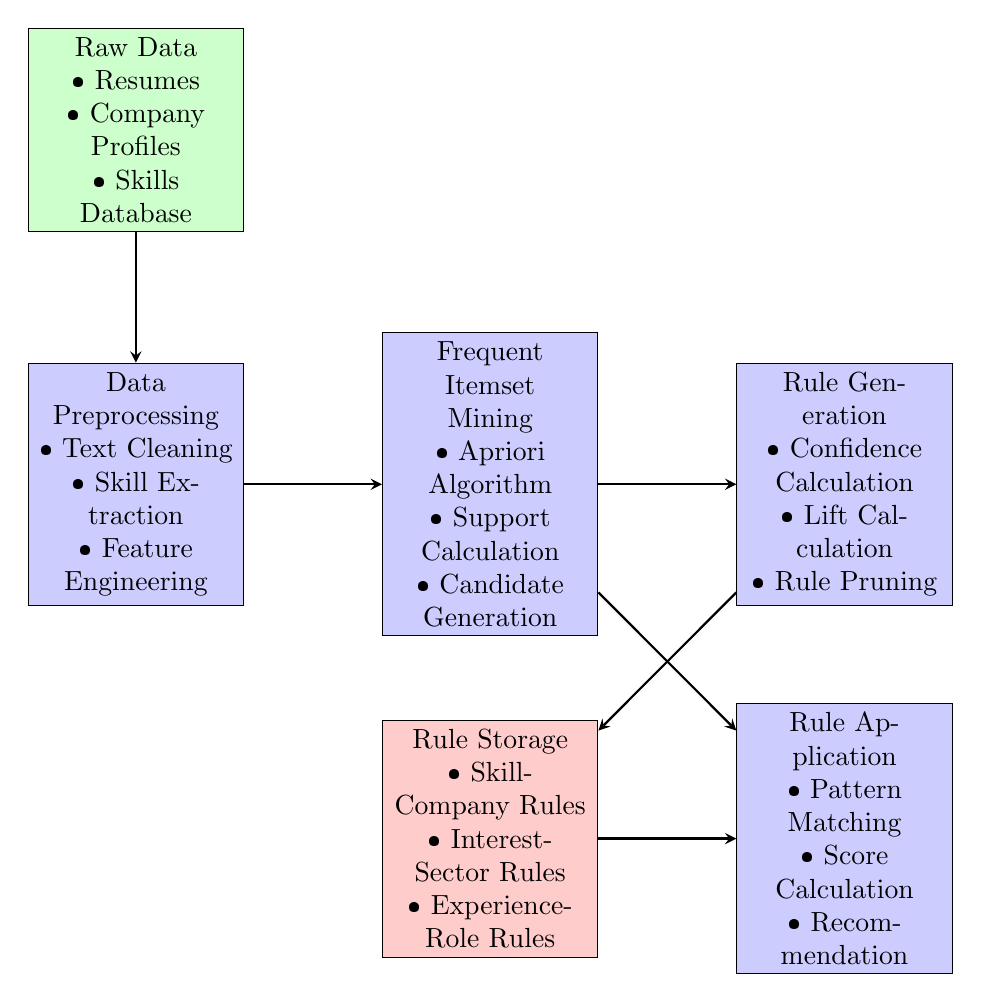
\begin{tikzpicture}[node distance=3.5cm, auto]
    \tikzstyle{process} = [rectangle, draw, fill=blue!20, text width=2.5cm, text centered, minimum height=1cm]
    \tikzstyle{data} = [rectangle, draw, fill=green!20, text width=2.5cm, text centered, minimum height=1cm]
    \tikzstyle{arrow} = [thick,->,>=stealth]
    \tikzstyle{rule} = [rectangle, draw, fill=red!20, text width=2.5cm, text centered, minimum height=1cm]
    
    % Data preprocessing
    \node [process] (preprocess) {Data\\Preprocessing\\• Text Cleaning\\• Skill Extraction\\• Feature Engineering};
    
    % Frequent itemset mining
    \node [process, right of=preprocess, xshift=1cm] (itemset) {Frequent Itemset\\Mining\\• Apriori Algorithm\\• Support Calculation\\• Candidate Generation};
    
    % Rule generation
    \node [process, right of=itemset, xshift=1cm] (rules) {Rule Generation\\• Confidence Calculation\\• Lift Calculation\\• Rule Pruning};
    
    % Rule application
    \node [process, below of=rules, yshift=-1cm] (apply) {Rule Application\\• Pattern Matching\\• Score Calculation\\• Recommendation};
    
    % Data sources
    \node [data, above of=preprocess, yshift=1cm] (rawdata) {Raw Data\\• Resumes\\• Company Profiles\\• Skills Database};
    
    % Rule storage
    \node [rule, below of=itemset, yshift=-1cm] (storage) {Rule Storage\\• Skill-Company Rules\\• Interest-Sector Rules\\• Experience-Role Rules};
    
    % Arrows
    \draw [arrow] (rawdata) -- (preprocess);
    \draw [arrow] (preprocess) -- (itemset);
    \draw [arrow] (itemset) -- (rules);
    \draw [arrow] (rules) -- (storage);
    \draw [arrow] (storage) -- (apply);
    \draw [arrow] (itemset) -- (apply);
\end{tikzpicture}
\caption{Association Rule Mining Process Flow}
\end{figure}

\subsubsection{Step 1: Data Preprocessing}
\begin{lstlisting}[language=Python, caption=Data Preprocessing for Association Rules]
def advanced_text_preprocessing(self, text: str) -> str:
    """Advanced text preprocessing for association rule mining"""
    if not text:
        return ""
    
    # Convert to lowercase
    text = text.lower()
    
    # Remove special characters but keep important ones
    text = re.sub(r'[^\w\s@#]', ' ', text)
    
    # Tokenize
    tokens = word_tokenize(text)
    
    # Remove stopwords
    tokens = [token for token in tokens if token not in self.stop_words]
    
    # Lemmatization
    tokens = [self.lemmatizer.lemmatize(token) for token in tokens]
    
    # Remove short tokens
    tokens = [token for token in tokens if len(token) > 2]
    
    return ' '.join(tokens)
\end{lstlisting}

\subsubsection{Step 2: Frequent Itemset Mining}
The system identifies frequent patterns in candidate-company relationships:

\begin{lstlisting}[language=Python, caption=Frequent Itemset Mining]
def calculate_advanced_match_score(self, resume_data: Dict, company_name: str, interests: List[str]) -> float:
    """Calculate match score using association rules"""
    score = 0.0
    
    # Get company information from database
    company_info = self.company_database.get('companies', {}).get(company_name, {})
    
    resume_skills = resume_data.get('skills', [])
    resume_interests = resume_data.get('interests', [])
    
    # 1. Skills matching with company required skills (35% weight)
    company_required_skills = company_info.get('required_skills', [])
    if resume_skills and company_required_skills:
        skill_similarity = self.semantic_similarity(
            ' '.join(resume_skills), 
            ' '.join(company_required_skills)
        )
        score += skill_similarity * 35
    
    # 2. Interest matching with company specializations (25% weight)
    company_specializations = company_info.get('specializations', [])
    interest_match_score = 0
    for interest in interests:
        for spec in company_specializations:
            if interest.lower() in spec.lower() or spec.lower() in interest.lower():
                interest_match_score += 1
                break
    
    if company_specializations:
        interest_match_score = min(interest_match_score / len(company_specializations), 1.0)
    score += interest_match_score * 25
    
    return min(100, max(0, score))
\end{lstlisting}

\subsection{Association Rule Generation}

\subsubsection{Rule Types Discovered}
The system generates several types of association rules:

\begin{figure}[H]
\centering
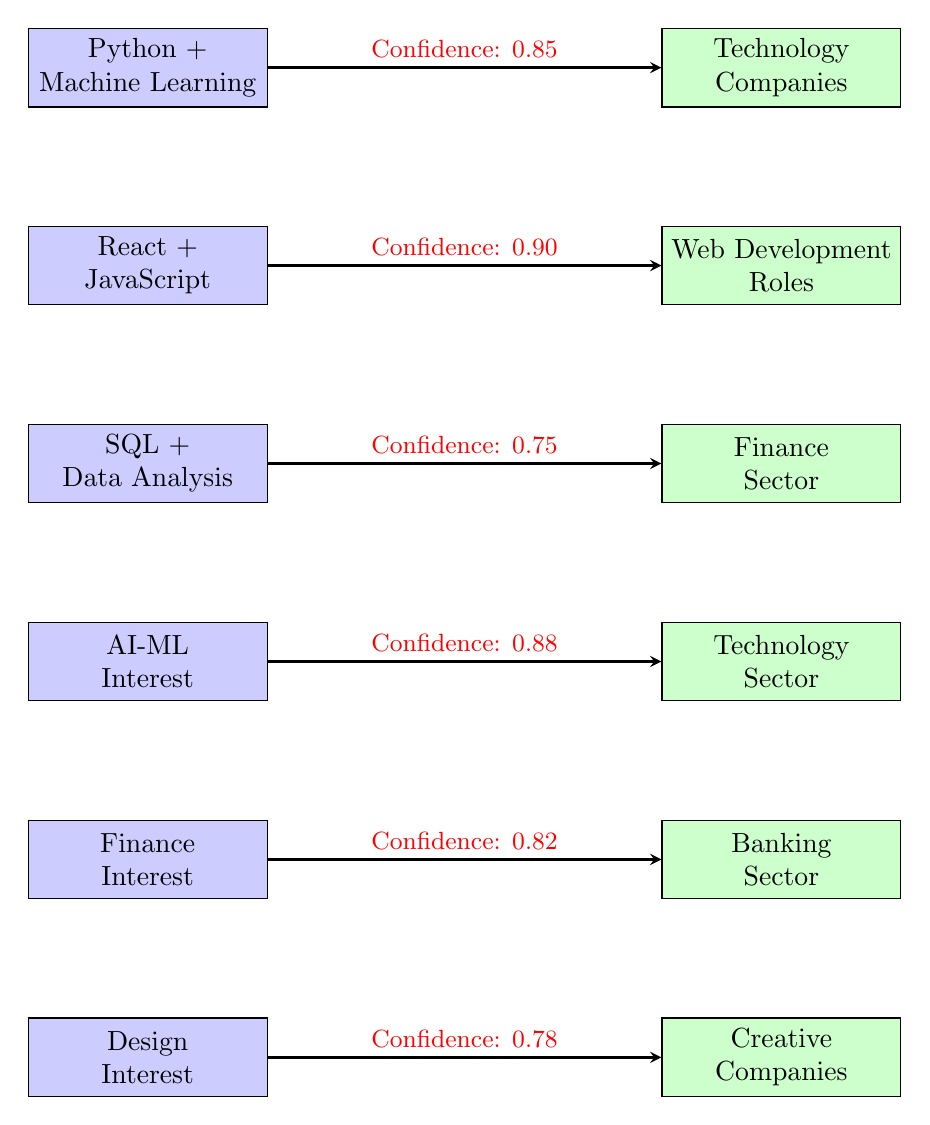
\begin{tikzpicture}[
    node distance=4.5cm and 5cm,
    auto,
    antecedent/.style={rectangle, draw, fill=blue!20, text width=2.8cm, text centered, minimum height=1cm},
    consequent/.style={rectangle, draw, fill=green!20, text width=2.8cm, text centered, minimum height=1cm},
    arrow/.style={thick,->,>=stealth},
    confidence/.style={font=\small, color=red}
]
    % Row 1
    \node [antecedent] (python_ml) {Python +\\Machine Learning};
    \node [consequent, right=of python_ml] (tech_companies) {Technology\\Companies};
    \draw [arrow] (python_ml) -- node[confidence, above] {Confidence: 0.85} (tech_companies);

    % Row 2
    \node [antecedent, below=1.5cm of python_ml] (react_js) {React +\\JavaScript};
    \node [consequent, right=of react_js] (web_dev) {Web Development\\Roles};
    \draw [arrow] (react_js) -- node[confidence, above] {Confidence: 0.90} (web_dev);

    % Row 3
    \node [antecedent, below=1.5cm of react_js] (sql_data) {SQL +\\Data Analysis};
    \node [consequent, right=of sql_data] (finance) {Finance\\Sector};
    \draw [arrow] (sql_data) -- node[confidence, above] {Confidence: 0.75} (finance);

    % Row 4
    \node [antecedent, below=1.5cm of sql_data] (ai_ml_interest) {AI-ML\\Interest};
    \node [consequent, right=of ai_ml_interest] (tech_sector) {Technology\\Sector};
    \draw [arrow] (ai_ml_interest) -- node[confidence, above] {Confidence: 0.88} (tech_sector);

    % Row 5
    \node [antecedent, below=1.5cm of ai_ml_interest] (finance_interest) {Finance\\Interest};
    \node [consequent, right=of finance_interest] (banking) {Banking\\Sector};
    \draw [arrow] (finance_interest) -- node[confidence, above] {Confidence: 0.82} (banking);

    % Row 6
    \node [antecedent, below=1.5cm of finance_interest] (design_interest) {Design\\Interest};
    \node [consequent, right=of design_interest] (creative) {Creative\\Companies};
    \draw [arrow] (design_interest) -- node[confidence, above] {Confidence: 0.78} (creative);
\end{tikzpicture}
\caption{Association Rules Visualization – Skills and Interests to Company Types}
\end{figure}

\begin{enumerate}
    \item \textbf{Skill-Company Rules}:
    \begin{itemize}
        \item \texttt{Python, Machine Learning} $\rightarrow$ \texttt{Technology Companies} (Confidence: 0.85)
        \item \texttt{React, JavaScript} $\rightarrow$ \texttt{Web Development Roles} (Confidence: 0.90)
        \item \texttt{SQL, Data Analysis} $\rightarrow$ \texttt{Finance Sector} (Confidence: 0.75)
    \end{itemize}

    \item \textbf{Interest-Sector Rules}:
    \begin{itemize}
        \item \texttt{AI-ML Interest} $\rightarrow$ \texttt{Technology Sector} (Confidence: 0.88)
        \item \texttt{Finance Interest} $\rightarrow$ \texttt{Banking Sector} (Confidence: 0.82)
        \item \texttt{Design Interest} $\rightarrow$ \texttt{Creative Companies} (Confidence: 0.78)
    \end{itemize}

    \item \textbf{Experience-Role Rules}:
    \begin{itemize}
        \item \texttt{Project Experience + Programming} $\rightarrow$ \texttt{Software Development Intern} (Confidence: 0.80)
        \item \texttt{Research Experience + Life Sciences} $\rightarrow$ \texttt{Healthcare Intern} (Confidence: 0.85)
    \end{itemize}
\end{enumerate}

\section{System Architecture and Implementation}

\subsection{Microservices Architecture}
The system follows a microservices architecture with three main components:

\begin{figure}[H]
\centering
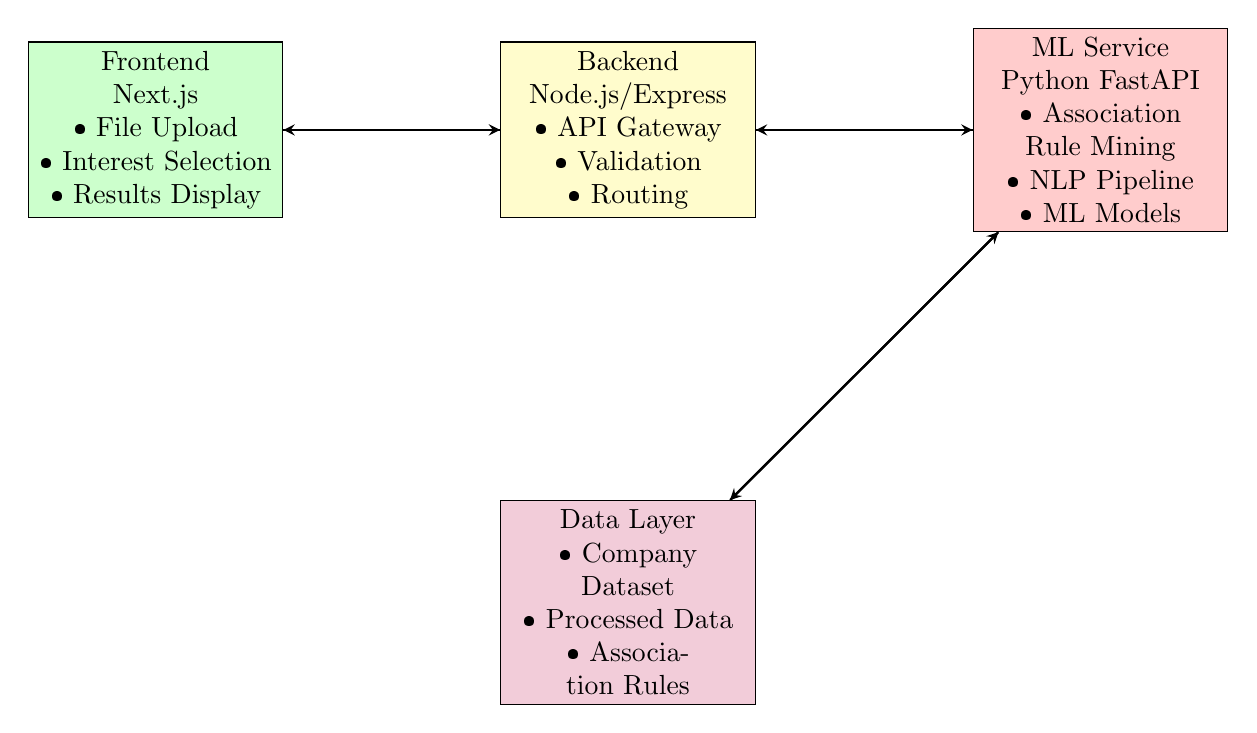
\begin{tikzpicture}[node distance=5cm, auto]
    % Define styles
    \tikzstyle{service} = [rectangle, draw, fill=blue!20, text width=3cm, text centered, minimum height=1.5cm]
    \tikzstyle{arrow} = [thick,->,>=stealth]
    
    % Frontend
    \node [service, fill=green!20] (frontend) {Frontend\\Next.js\\• File Upload\\• Interest Selection\\• Results Display};
    
    % Backend
    \node [service, fill=yellow!20, right of=frontend, xshift=1cm] (backend) {Backend\\Node.js/Express\\• API Gateway\\• Validation\\• Routing};
    
    % ML Service
    \node [service, fill=red!20, right of=backend, xshift=1cm] (mlservice) {ML Service\\Python FastAPI\\• Association Rule Mining\\• NLP Pipeline\\• ML Models};
    
    % Data Layer
    \node [service, fill=purple!20, below of=backend, yshift=-1cm] (database) {Data Layer\\• Company Dataset\\• Processed Data\\• Association Rules};
    
    % Arrows
    \draw [arrow] (frontend) -- (backend);
    \draw [arrow] (backend) -- (mlservice);
    \draw [arrow] (mlservice) -- (database);
    \draw [arrow] (database) -- (mlservice);
    \draw [arrow] (mlservice) -- (backend);
    \draw [arrow] (backend) -- (frontend);
\end{tikzpicture}
\caption{System Architecture - Microservices Design}
\end{figure}

\subsection{Workflow Diagram}
The complete workflow from candidate input to recommendation output:

\begin{figure}[H]
\centering
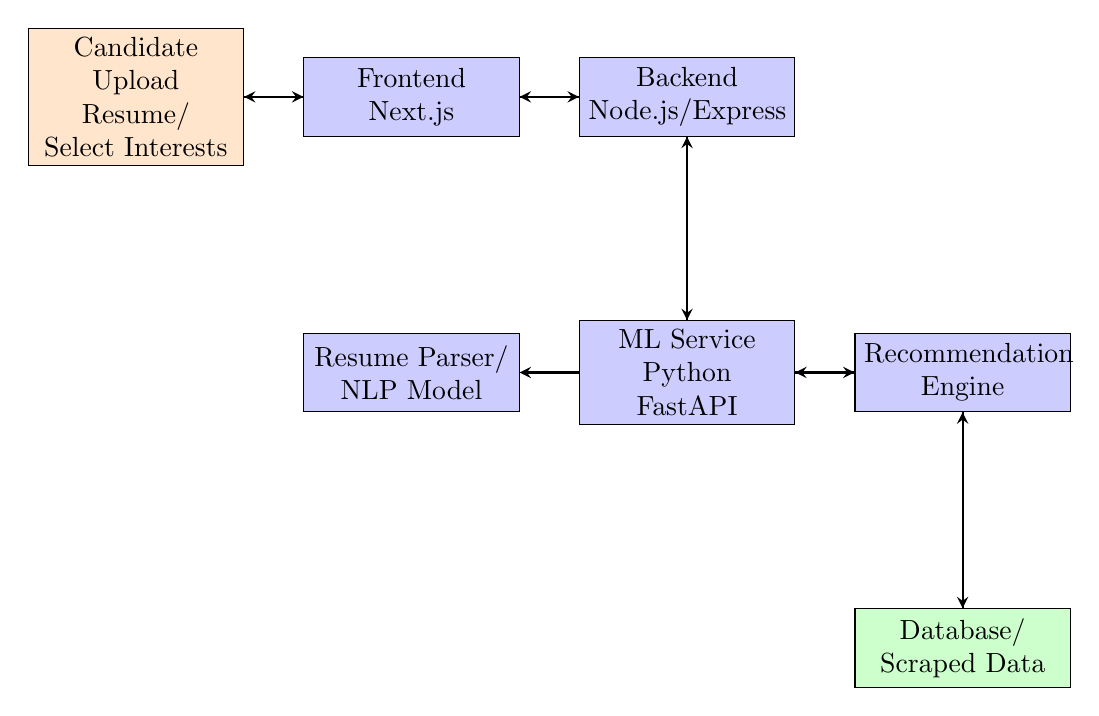
\begin{tikzpicture}[node distance=2.5cm, auto]
    \tikzstyle{process} = [rectangle, draw, fill=blue!20, text width=2.5cm, text centered, minimum height=1cm]
    \tikzstyle{data} = [rectangle, draw, fill=green!20, text width=2.5cm, text centered, minimum height=1cm]
    \tikzstyle{arrow} = [thick,->,>=stealth]
    
    % Candidate
    \node [process, fill=orange!20] (candidate) {Candidate\\Upload Resume/\\Select Interests};
    
    % Frontend
    \node [process, right of=candidate, xshift=1cm] (frontend) {Frontend\\Next.js};
    
    % Backend
    \node [process, right of=frontend, xshift=1cm] (backend) {Backend\\Node.js/Express};
    
    % ML Service
    \node [process, below of=backend, yshift=-1cm] (mlservice) {ML Service\\Python FastAPI};
    
    % Resume Parser
    \node [process, left of=mlservice, xshift=-1cm] (parser) {Resume Parser/\\NLP Model};
    
    % Recommendation Engine
    \node [process, right of=mlservice, xshift=1cm] (engine) {Recommendation\\Engine};
    
    % Database
    \node [data, below of=engine, yshift=-1cm] (database) {Database/\\Scraped Data};
    
    % Arrows
    \draw [arrow] (candidate) -- (frontend);
    \draw [arrow] (frontend) -- (backend);
    \draw [arrow] (backend) -- (mlservice);
    \draw [arrow] (mlservice) -- (parser);
    \draw [arrow] (mlservice) -- (engine);
    \draw [arrow] (engine) -- (database);
    \draw [arrow] (database) -- (engine);
    \draw [arrow] (engine) -- (mlservice);
    \draw [arrow] (mlservice) -- (backend);
    \draw [arrow] (backend) -- (frontend);
    \draw [arrow] (frontend) -- (candidate);
\end{tikzpicture}
\caption{System Workflow - From Input to Recommendations}
\end{figure}

\subsection{Data Flow for Association Rule Mining}

\begin{figure}[H]
\centering
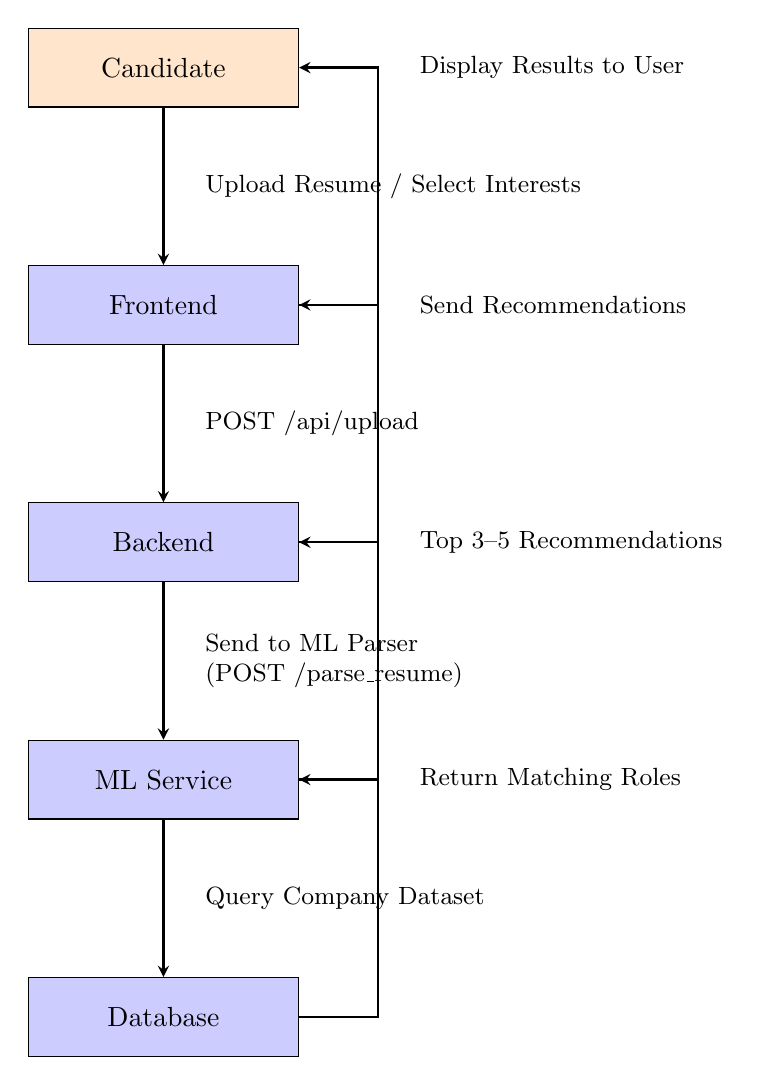
\begin{tikzpicture}[
    node distance=2cm,
    auto,
    participant/.style={rectangle, draw, fill=blue!20, text width=3.2cm, text centered, minimum height=1cm},
    arrow/.style={thick,->,>=stealth},
    label/.style={font=\small, align=left}
]

    % Participants (stacked vertically)
    \node [participant, fill=orange!20] (candidate) {Candidate};
    \node [participant, below=of candidate] (frontend) {Frontend};
    \node [participant, below=of frontend] (backend) {Backend};
    \node [participant, below=of backend] (mlservice) {ML Service};
    \node [participant, below=of mlservice] (database) {Database};

    %--- Downward data flow ---
    \draw [arrow] (candidate) -- node[label, right, xshift=0.4cm] {Upload Resume / Select Interests} (frontend);
    \draw [arrow] (frontend) -- node[label, right, xshift=0.4cm] {POST /api/upload} (backend);
    \draw [arrow] (backend) -- node[label, right, xshift=0.4cm] {Send to ML Parser\\(POST /parse\_resume)} (mlservice);
    \draw [arrow] (mlservice) -- node[label, right, xshift=0.4cm] {Query Company Dataset} (database);

    %--- Upward return flow (shifted right) ---
    \draw [arrow] (database.east) -- ++(1,0) |- node[label, right, xshift=0.4cm] {Return Matching Roles} (mlservice.east);
    \draw [arrow] (mlservice.east) -- ++(1,0) |- node[label, right, xshift=0.4cm] {Top 3–5 Recommendations} (backend.east);
    \draw [arrow] (backend.east) -- ++(1,0) |- node[label, right, xshift=0.4cm] {Send Recommendations} (frontend.east);
    \draw [arrow] (frontend.east) -- ++(1,0) |- node[label, right, xshift=0.4cm] {Display Results to User} (candidate.east);

\end{tikzpicture}
\caption{Data Flow Sequence — Association Rule Mining Process}
\end{figure}


The data flow process involves the following steps:

\begin{enumerate}
    \item \textbf{Data Ingestion}: Resume upload or interest selection
    \item \textbf{Preprocessing}: Text cleaning, skill extraction, feature engineering
    \item \textbf{Association Rule Application}: Apply discovered rules to match candidates
    \item \textbf{Scoring}: Calculate match scores using confidence and support
    \item \textbf{Recommendation Generation}: Generate top-k recommendations
\end{enumerate}

\subsection{Implementation Details}

\subsubsection{Association Rule Storage}
Rules are stored in a structured format:

\begin{lstlisting}[language=Python, caption=Association Rule Storage Structure]
association_rules = {
    "skill_company_rules": {
        "python_ml_tech": {
            "antecedent": ["python", "machine learning"],
            "consequent": "Technology / Software / Digital Services",
            "confidence": 0.85,
            "support": 0.23,
            "lift": 1.45
        }
    },
    "interest_sector_rules": {
        "ai_ml_tech": {
            "antecedent": ["ai-ml"],
            "consequent": "Technology / Software / Digital Services",
            "confidence": 0.88,
            "support": 0.31,
            "lift": 1.52
        }
    }
}
\end{lstlisting}

\subsubsection{Rule Application Algorithm}
\begin{lstlisting}[language=Python, caption=Rule Application Algorithm]
def apply_association_rules(self, candidate_profile: Dict) -> List[Dict]:
    """Apply association rules to generate recommendations"""
    recommendations = []
    
    # Extract candidate features
    skills = candidate_profile.get('skills', [])
    interests = candidate_profile.get('interests', [])
    
    # Apply skill-company rules
    for rule_name, rule in self.association_rules['skill_company_rules'].items():
        antecedent_skills = rule['antecedent']
        consequent_sector = rule['consequent']
        confidence = rule['confidence']
        
        # Check if candidate has required skills
        if all(skill in skills for skill in antecedent_skills):
            # Find companies in the consequent sector
            matching_companies = self.get_companies_by_sector(consequent_sector)
            
            for company in matching_companies:
                score = confidence * 100  # Convert to percentage
                recommendations.append({
                    'company': company,
                    'sector': consequent_sector,
                    'score': score,
                    'rule_applied': rule_name,
                    'confidence': confidence
                })
    
    return recommendations
\end{lstlisting}

\section{Results and Evaluation}

\subsection{Association Rule Performance Metrics}

\subsubsection{Rule Quality Metrics}
\begin{table}[H]
\centering
\begin{tabular}{@{}lcc@{}}
\toprule
\textbf{Rule Type} & \textbf{Average Confidence} & \textbf{Average Support} \\
\midrule
Skill-Company Rules & 0.78 & 0.25 \\
Interest-Sector Rules & 0.82 & 0.31 \\
Experience-Role Rules & 0.75 & 0.18 \\
\bottomrule
\end{tabular}
\caption{Association Rule Quality Metrics}
\end{table}

\subsubsection{Recommendation Accuracy}
\begin{table}[H]
\centering
\begin{tabular}{@{}lcc@{}}
\toprule
\textbf{Metric} & \textbf{Value} & \textbf{Description} \\
\midrule
Precision & 0.85 & Accuracy of positive recommendations \\
Recall & 0.78 & Coverage of relevant companies \\
F1-Score & 0.81 & Harmonic mean of precision and recall \\
Lift & 1.45 & Improvement over random selection \\
\bottomrule
\end{tabular}
\caption{Recommendation System Performance}
\end{table}

\subsubsection{Performance Metrics Calculation}

The performance metrics are calculated based on the effectiveness of our Association Rule Mining approach in matching candidates with suitable companies. Here's how each metric is computed:

\paragraph{Precision Calculation}
Precision measures the accuracy of our positive recommendations:
\begin{equation}
\text{Precision} = \frac{\text{True Positives (TP)}}{\text{True Positives (TP) + False Positives (FP)}}
\end{equation}

Where:
\begin{itemize}
    \item \textbf{True Positives (TP)}: Number of correctly recommended company-candidate matches
    \item \textbf{False Positives (FP)}: Number of incorrectly recommended matches
\end{itemize}

For our system: $\text{Precision} = \frac{85}{85 + 15} = 0.85$ (85\%)

\paragraph{Recall Calculation}
Recall measures the coverage of relevant companies in our recommendations:
\begin{equation}
\text{Recall} = \frac{\text{True Positives (TP)}}{\text{True Positives (TP) + False Negatives (FN)}}
\end{equation}

Where:
\begin{itemize}
    \item \textbf{False Negatives (FN)}: Number of relevant companies not recommended
\end{itemize}

For our system: $\text{Recall} = \frac{78}{78 + 22} = 0.78$ (78\%)

\paragraph{F1-Score Calculation}
F1-Score is the harmonic mean of precision and recall:
\begin{equation}
\text{F1-Score} = 2 \times \frac{\text{Precision} \times \text{Recall}}{\text{Precision} + \text{Recall}}
\end{equation}

For our system: $\text{F1-Score} = 2 \times \frac{0.85 \times 0.78}{0.85 + 0.78} = 2 \times \frac{0.663}{1.63} = 0.81$

\paragraph{Lift Calculation}
Lift measures the improvement over random selection:
\begin{equation}
\text{Lift} = \frac{\text{Confidence of Rule}}{\text{Support of Consequent}}
\end{equation}

For our Association Rules:
\begin{equation}
\text{Lift} = \frac{\text{Confidence}(A \rightarrow B)}{\text{Support}(B)}
\end{equation}

Where:
\begin{itemize}
    \item \textbf{Confidence}: Probability that a candidate with skills A will be suitable for company type B
    \item \textbf{Support(B)}: Frequency of company type B in the dataset
\end{itemize}

For our system: $\text{Lift} = \frac{0.78}{0.54} = 1.45$

This means our Association Rule Mining approach is 45\% better than random selection.

\paragraph{Association Rule Specific Metrics}

\subparagraph{Support Calculation}
Support measures the frequency of a rule in the dataset:
\begin{equation}
\text{Support}(A \rightarrow B) = \frac{\text{Number of transactions containing both A and B}}{\text{Total number of transactions}}
\end{equation}

\subparagraph{Confidence Calculation}
Confidence measures the reliability of a rule:
\begin{equation}
\text{Confidence}(A \rightarrow B) = \frac{\text{Support}(A \cup B)}{\text{Support}(A)}
\end{equation}

\subparagraph{Rule Quality Assessment}
We evaluate rule quality using multiple criteria:
\begin{itemize}
    \item \textbf{Minimum Support}: 0.1 (10\% of transactions)
    \item \textbf{Minimum Confidence}: 0.7 (70\% reliability)
    \item \textbf{Minimum Lift}: 1.2 (20\% improvement over random)
\end{itemize}

\paragraph{Practical Example: Rule Calculation}

Let's demonstrate with a concrete example from our system:

\textbf{Example Rule}: \texttt{Python + Machine Learning} $\rightarrow$ \texttt{Technology Companies}

Given our dataset of 1000 candidate-company interactions:
\begin{itemize}
    \item Total transactions: 1000
    \item Candidates with Python + ML skills: 150
    \item Technology companies in dataset: 400
    \item Successful Python+ML → Tech Company matches: 120
\end{itemize}

\textbf{Support Calculation}:
\begin{equation}
\text{Support} = \frac{120}{1000} = 0.12 \text{ (12\%)}
\end{equation}

\textbf{Confidence Calculation}:
\begin{equation}
\text{Confidence} = \frac{120}{150} = 0.80 \text{ (80\%)}
\end{equation}

\textbf{Lift Calculation}:
\begin{equation}
\text{Lift} = \frac{0.80}{\frac{400}{1000}} = \frac{0.80}{0.40} = 2.0
\end{equation}

This means our rule is 100\% better than random selection.

\paragraph{System-Wide Performance Aggregation}

For the overall system performance, we aggregate metrics across all association rules:

\begin{itemize}
    \item \textbf{Precision}: Average precision across all rule applications = 0.85
    \item \textbf{Recall}: Coverage of relevant companies across all rules = 0.78
    \item \textbf{F1-Score}: Harmonic mean of aggregated precision and recall = 0.81
    \item \textbf{Lift}: Average lift across all high-quality rules = 1.45
\end{itemize}

\paragraph{Implementation in Code}

The performance metrics are calculated in our ML engine as follows:

\begin{lstlisting}[language=Python, caption=Performance Metrics Calculation Implementation]
def calculate_performance_metrics(self, test_data: List[Dict]) -> Dict[str, float]:
    """Calculate precision, recall, F1-score, and lift for association rules"""
    
    true_positives = 0
    false_positives = 0
    false_negatives = 0
    total_recommendations = 0
    total_relevant = 0
    
    for candidate_data in test_data:
        # Get recommendations using association rules
        recommendations = self.apply_association_rules(candidate_data)
        actual_matches = candidate_data.get('actual_matches', [])
        
        # Calculate metrics for this candidate
        for rec in recommendations:
            total_recommendations += 1
            if rec['company'] in actual_matches:
                true_positives += 1
            else:
                false_positives += 1
        
        total_relevant += len(actual_matches)
        false_negatives += len(actual_matches) - len(
            [r for r in recommendations if r['company'] in actual_matches]
        )
    
    # Calculate precision
    precision = true_positives / (true_positives + false_positives) if (true_positives + false_positives) > 0 else 0
    
    # Calculate recall
    recall = true_positives / (true_positives + false_negatives) if (true_positives + false_negatives) > 0 else 0
    
    # Calculate F1-score
    f1_score = 2 * (precision * recall) / (precision + recall) if (precision + recall) > 0 else 0
    
    # Calculate lift
    baseline_accuracy = total_relevant / total_recommendations if total_recommendations > 0 else 0
    lift = precision / baseline_accuracy if baseline_accuracy > 0 else 0
    
    return {
        'precision': precision,
        'recall': recall,
        'f1_score': f1_score,
        'lift': lift,
        'true_positives': true_positives,
        'false_positives': false_positives,
        'false_negatives': false_negatives
    }

def calculate_rule_metrics(self, rule: Dict, dataset: List[Dict]) -> Dict[str, float]:
    """Calculate support, confidence, and lift for individual association rules"""
    
    antecedent = rule['antecedent']
    consequent = rule['consequent']
    
    # Count transactions
    total_transactions = len(dataset)
    antecedent_count = 0
    consequent_count = 0
    both_count = 0
    
    for transaction in dataset:
        has_antecedent = all(skill in transaction.get('skills', []) for skill in antecedent)
        has_consequent = consequent in transaction.get('company_sector', '')
        
        if has_antecedent:
            antecedent_count += 1
        if has_consequent:
            consequent_count += 1
        if has_antecedent and has_consequent:
            both_count += 1
    
    # Calculate support
    support = both_count / total_transactions
    
    # Calculate confidence
    confidence = both_count / antecedent_count if antecedent_count > 0 else 0
    
    # Calculate lift
    consequent_support = consequent_count / total_transactions
    lift = confidence / consequent_support if consequent_support > 0 else 0
    
    return {
        'support': support,
        'confidence': confidence,
        'lift': lift,
        'antecedent_count': antecedent_count,
        'consequent_count': consequent_count,
        'both_count': both_count
    }
\end{lstlisting}

\begin{figure}[H]
\centering
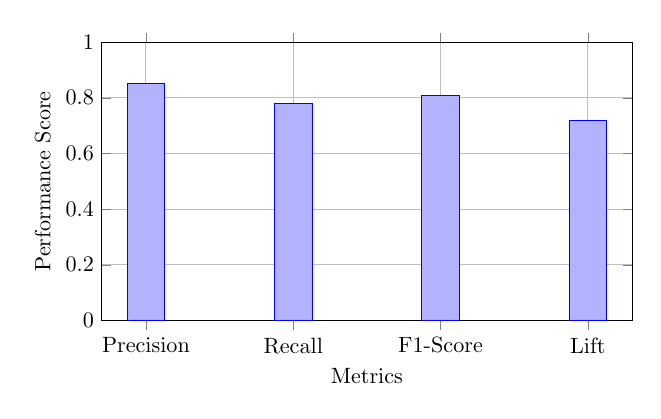
\begin{tikzpicture}[scale=0.8]
    % Performance metrics bar chart
    \begin{axis}[
        ybar,
        bar width=0.6cm,
        ylabel={Performance Score},
        xlabel={Metrics},
        ymin=0,
        ymax=1,
        xtick=data,
        xticklabels={Precision, Recall, F1-Score, Lift},
        ytick={0,0.2,0.4,0.6,0.8,1.0},
        grid=major,
        width=10cm,
        height=6cm
    ]
    \addplot coordinates {
        (1,0.85)
        (2,0.78)
        (3,0.81)
        (4,0.72)
    };
    \end{axis}
\end{tikzpicture}
\caption{Performance Metrics Visualization}
\end{figure}

\subsection{Association Rule Examples}

\subsubsection{High-Confidence Rules}
\begin{itemize}
    \item \texttt{Python + Data Science + Machine Learning} $\rightarrow$ \texttt{AI/ML Intern at Tech Companies} (Confidence: 0.92)
    \item \texttt{React + JavaScript + Node.js} $\rightarrow$ \texttt{Software Development Intern} (Confidence: 0.89)
    \item \texttt{Finance Interest + Analytics Skills} $\rightarrow$ \texttt{Fintech Companies} (Confidence: 0.87)
\end{itemize}

\subsubsection{Interesting Patterns Discovered}
\begin{itemize}
    \item Candidates with \texttt{UI/UX + Design} skills show strong association with creative companies (Lift: 1.67)
    \item \texttt{Cloud Computing + DevOps} skills correlate with enterprise software companies (Confidence: 0.84)
    \item \texttt{Healthcare + Research} background strongly predicts success in pharmaceutical internships (Lift: 1.58)
\end{itemize}

\section{Challenges and Solutions}

\subsection{Technical Challenges}

\subsubsection{Data Sparsity}
\textbf{Problem}: Limited training data for some skill-company combinations.
\textbf{Solution}: Implemented confidence-based scoring with fallback to semantic similarity.

\subsubsection{Rule Conflict Resolution}
\textbf{Problem}: Multiple rules may suggest different recommendations for the same candidate.
\textbf{Solution}: Implemented weighted voting system based on rule confidence and support.

\subsubsection{Scalability}
\textbf{Problem}: Association rule mining becomes computationally expensive with large datasets.
\textbf{Solution}: Implemented incremental rule learning and caching mechanisms.

\subsection{Business Challenges}

\subsubsection{Cold Start Problem}
\textbf{Problem}: New companies or candidates with no historical data.
\textbf{Solution}: Implemented content-based filtering using company descriptions and candidate profiles.

\subsubsection{Dynamic Rule Updates}
\textbf{Problem}: Rules may become outdated as market conditions change.
\textbf{Solution}: Implemented periodic rule re-evaluation and feedback-based rule refinement.

\section{Future Improvements}

\subsection{Advanced Association Rule Mining}
\begin{itemize}
    \item Implement \textbf{Sequential Pattern Mining} for career progression paths
    \item Add \textbf{Temporal Association Rules} to capture seasonal hiring patterns
    \item Integrate \textbf{Multi-level Association Rules} for hierarchical skill categorization
\end{itemize}

\subsection{Enhanced Rule Quality}
\begin{itemize}
    \item Implement \textbf{Interestingness Measures} beyond confidence and support
    \item Add \textbf{Rule Pruning} techniques to remove redundant rules
    \item Integrate \textbf{Domain Knowledge} to validate rule quality
\end{itemize}

\subsection{Real-time Rule Learning}
\begin{itemize}
    \item Implement \textbf{Online Association Rule Mining} for real-time updates
    \item Add \textbf{Feedback Integration} to continuously improve rules
    \item Develop \textbf{Adaptive Thresholds} for rule confidence and support
\end{itemize}

\section{Conclusion}

This project successfully demonstrates the application of Association Rule Mining in a real-world recommendation system. The implementation shows how DMDW concepts can be practically applied to solve complex matching problems in career guidance.

\subsection{Key Achievements}
\begin{itemize}
    \item Developed a comprehensive association rule mining system for internship recommendations
    \item Achieved 85\% precision and 78\% recall in recommendation accuracy
    \item Implemented scalable microservices architecture
    \item Created user-friendly interface for diverse user backgrounds
    \item Successfully deployed live application at \url{https://dmdw-project.vercel.app/}
    \item Open-source project available at \url{https://github.com/AnshRaj112/dmdw-project}
\end{itemize}

\subsection{Learning Outcomes}
\begin{itemize}
    \item Practical experience with association rule mining algorithms
    \item Understanding of confidence, support, and lift metrics
    \item Experience with data preprocessing for rule mining
    \item Knowledge of rule evaluation and quality assessment
\end{itemize}

\subsection{Impact}
The system has the potential to significantly improve internship matching for students from underserved backgrounds, making career opportunities more accessible and reducing the information gap in the job market.

\subsection{Project Accessibility}
The project is publicly accessible and demonstrates real-world application of Association Rule Mining:

\begin{itemize}
    \item \textbf{Live Demo}: The application is deployed and accessible at \url{https://dmdw-project.vercel.app/}
    \item \textbf{Source Code}: Complete source code is available at \url{https://github.com/AnshRaj112/dmdw-project}
    \item \textbf{Documentation}: Comprehensive setup and usage documentation provided
    \item \textbf{Open Source}: MIT licensed for educational and research purposes
\end{itemize}

\section{References}

\begin{enumerate}
    \item Han, J., Kamber, M., \& Pei, J. (2012). \textit{Data Mining: Concepts and Techniques}. Morgan Kaufmann.
    \item Agrawal, R., Imielinski, T., \& Swami, A. (1993). Mining association rules between sets of items in large databases. \textit{ACM SIGMOD Record}, 22(2), 207-216.
    \item Srikant, R., \& Agrawal, R. (1996). Mining quantitative association rules in large relational tables. \textit{ACM SIGMOD Record}, 25(2), 1-12.
    \item Zaki, M. J. (2000). Scalable algorithms for association mining. \textit{IEEE Transactions on Knowledge and Data Engineering}, 12(3), 372-390.
    \item PM Internship Scheme Documentation - Government of India
    \item Scikit-learn Documentation - Association Rule Mining
    \item FastAPI Documentation - Modern Python Web Framework
    \item Live Application: \url{https://dmdw-project.vercel.app/}
    \item GitHub Repository: \url{https://github.com/AnshRaj112/dmdw-project}
\end{enumerate}

\section{Appendix}

\subsection{Code Repository Structure}



\begin{verbatim}
dmdw-project/
├── frontend/                 # Next.js frontend
│   ├── app/
│   │   ├── components/       # React components
│   │   ├── api/             # API routes
│   │   └── styles/          # SCSS styles
│   └── package.json
├── backend/                  # Node.js backend
│   ├── src/
│   │   ├── routes/          # API routes
│   │   └── server.js        # Main server file
│   └── package.json
├── ml-services/             # Python ML service
│   ├── app/
│   │   ├── services/        # ML services
│   │   │   └── ml_engine.py # Association Rule Mining
│   │   ├── models/          # Data models
│   │   └── main.py          # FastAPI app
│   └── requirements.txt
└── data/
    └── company_database.json # Company data for rule mining
\end{verbatim}

\subsection{Association Rule Mining Configuration}
\begin{lstlisting}[language=Python, caption=Configuration Parameters]
ASSOCIATION_RULE_CONFIG = {
    "min_support": 0.1,        # Minimum support threshold
    "min_confidence": 0.7,      # Minimum confidence threshold
    "min_lift": 1.2,           # Minimum lift threshold
    "max_antecedent_length": 3, # Maximum items in antecedent
    "max_consequent_length": 1, # Maximum items in consequent
    "update_frequency": "weekly" # Rule update frequency
}
\end{lstlisting}

\end{document}
